\documentclass{article}%
\usepackage[T1]{fontenc}%
\usepackage[utf8]{inputenc}%
\usepackage{lmodern}%
\usepackage{textcomp}%
\usepackage{lastpage}%
\usepackage[head=40pt,margin=0.5in,bottom=0.6in]{geometry}%
\usepackage{graphicx}%
%
\title{\textbf{69\% de los alimentos CLAP provienen de Turquía}}%
\author{El Nacional Web}%
\date{16/09/2018}%
%
\begin{document}%
\normalsize%
\maketitle%
\textbf{URL: }%
http://www.el{-}nacional.com/noticias/economia/los{-}alimentos{-}clap{-}provienen{-}turquia\_251966\newline%
%
\textbf{Periodico: }%
EN, %
ID: %
251966, %
Seccion: %
Economía\newline%
%
\textbf{Palabras Claves: }%
Economía\newline%
%
\textbf{Derecho: }%
2.10, %
Otros Derechos: %
, %
Sub Derechos: %
2.10.1.1\newline%
%
\textbf{EP: }%
NO\newline%
\newline%
%
\textbf{\textit{Los registros de movimientos aduanales mostraron que los productos turcos que ingresaron al país entre junio y agosto fueron traidos desde Estambul y Ankara~hasta el puerto~Cristóbal en Panamá y, posteriormente, al terminal portuario ubicado en el litoral central venezolano}}%
\newline%
\newline%
%
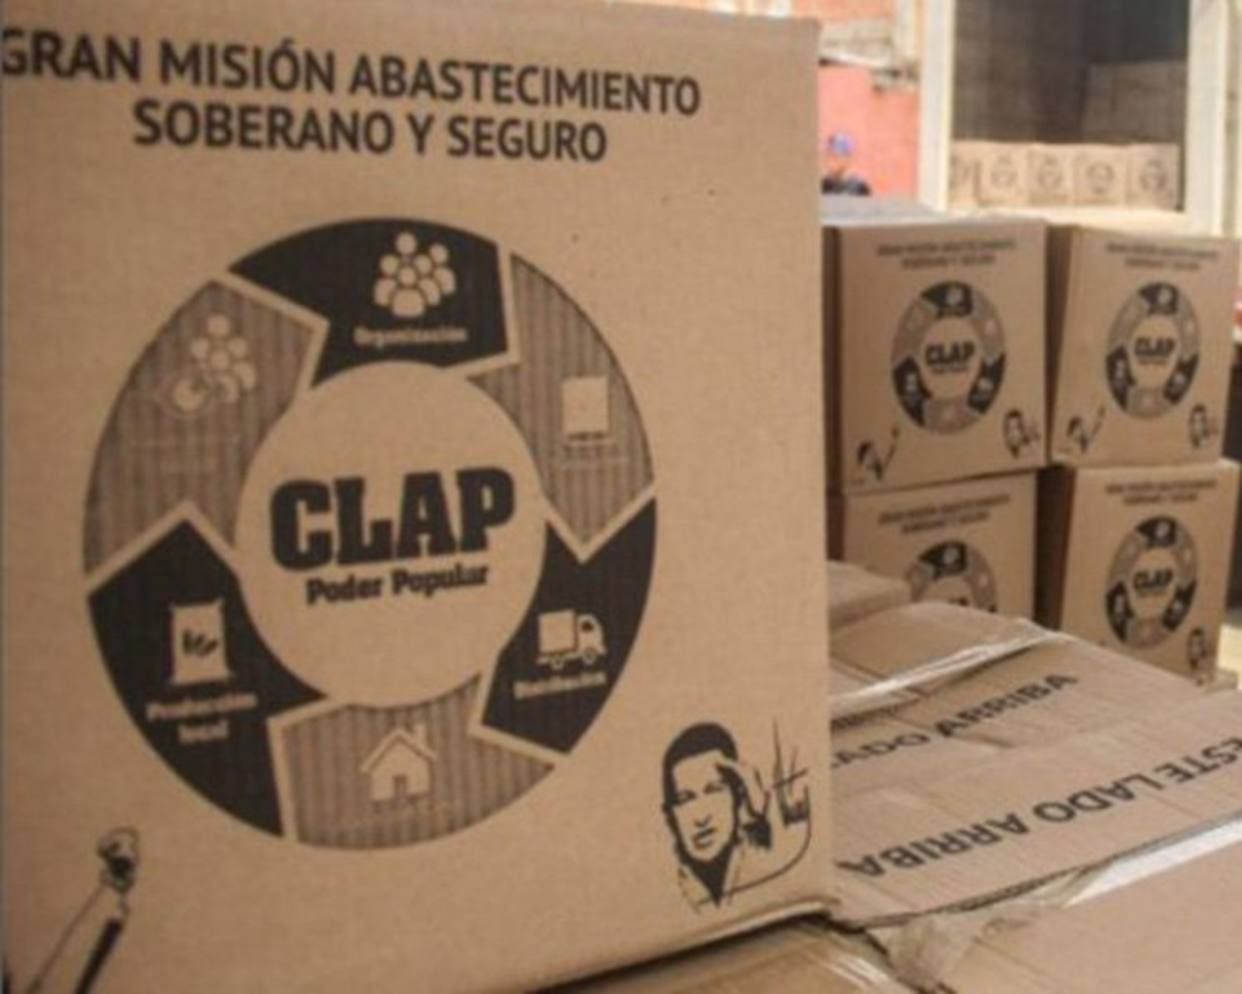
\includegraphics[width=300px]{21.jpg}%
\newline%
%
Los Comités Locales de Abastecimiento y Producción (CLAP) introdujeron~el último año alimentos~provenientes de Turquía importada mediante la empresa Corporación~Única de Servicios Productivos y Alimentarios C.A. (Cuspalca) y están llegando al puerto desde abril en la Guaira (Vargas).%
\newline%
%
Los registros indicaron que 69\% de la comida arribada a la entidad para ser entregada en la bodega de almacenaje del CLAP~provino de Turquía y 31\% de los productos eran de México, Brasil, Uruguay y Panamá, así lo reseñó~El Pitazo.%
\newline%
%
"Venezuela está convirtiendo a Turquía y a sus empresas en un intermediario que sirva como vía para evadir las medidas sancionatorias de Estados Unidos, al tiempo que políticamente se da pie a estas importaciones para fortalecer la geopolítica que impulsa el gobierno de Maduro, convirtiendo a Turquía en el nuevo aliado estratégico”, explicó~Ronald Rivas, economista.%
\newline%
%
Jorge Arreaza, canciller venezolano,~indicó que el gobierno considera a Turquía como un país aliado que ayuda a romper con el bloqueo expulsado por EE UU.%
\newline%
%
The Observatory of Economic Complexity, dedicada al registro de datos de comercio internacional, Turquía se posicionó durante el año 2017 como la 29º economía de exportación en el mundo.%
\newline%
%
“Los productos de la caja cambian de nacionalidad, pero el esquema de intermediarios parece ser una fórmula fija para la importación de alimentos para ser distribuidos por los CLAP”, concluye Rivas.%
\newline%
%
Algunos productos registran su origen en los empaques: leche de Alemania, caraotas negras de Etiopia, azúcar de Bélgica, arroz de Tailandia, lentejas de Canadá. Todas importadas, transportadas y empaquetadas a través de la empresa Yayla Agro Food Industry \& Transport Co, de capital turco y con 26 años de experiencia.%
\newline%
%
La nueva gama de productos provienen del país turco, pero no son fabricados por él, sino importados de países europeos, africanos y asiáticos.%
\newline%
%
Los registros de movimientos aduanales registraron que los productos turcos que ingresaron al país entre junio y agosto fueron traidos desde Estambul y Ankara~hasta el puerto~Cristóbal en Panamá y, posteriormente, al terminal portuario ubicado en el litoral central venezolano.%
\newline%
%
\end{document}